%%%%%%%%%%%%%%%%%%%%%%%%%%%%%%%%%%%%%%%%%
% Stylish Article
% LaTeX Template
% Version 2.1 (1/10/15)
%
% This template has been downloaded from:
% http://www.LaTeXTemplates.com
%
% Original author:
% Mathias Legrand (legrand.mathias@gmail.com) 
% With extensive modifications by:
% Vel (vel@latextemplates.com)
%
% License:
% CC BY-NC-SA 3.0 (http://creativecommons.org/licenses/by-nc-sa/3.0/)
%
%%%%%%%%%%%%%%%%%%%%%%%%%%%%%%%%%%%%%%%%%

%----------------------------------------------------------------------------------------
%	PACKAGES AND OTHER DOCUMENT CONFIGURATIONS
%----------------------------------------------------------------------------------------

\documentclass[fleqn,10pt]{UserGuideArx} % Document font size and equations flushed left

\usepackage[T1]{fontenc}

% \usepackage{microtype}
\usepackage{amsmath}
\usepackage[linesnumbered,ruled]{algorithm2e}

\usepackage[english]{babel} % Specify a different language here - english by default

\usepackage{lipsum} % Required to insert dummy text. To be removed otherwise

%----------------------------------------------------------------------------------------
%	COLUMNS
%----------------------------------------------------------------------------------------

\setlength{\columnsep}{0.55cm} % Distance between the two columns of text
\setlength{\fboxrule}{0.75pt} % Width of the border around the abstract

%----------------------------------------------------------------------------------------
%	COLORS
%----------------------------------------------------------------------------------------

\definecolor{color1}{RGB}{0,0,90} % Color of the article title and sections
\definecolor{color2}{RGB}{0,20,20} % Color of the boxes behind the abstract and headings

%----------------------------------------------------------------------------------------
%	HYPERLINKS
%----------------------------------------------------------------------------------------

\usepackage{hyperref} % Required for hyperlinks
\hypersetup{hidelinks,colorlinks,breaklinks=true,urlcolor=color2,citecolor=color1,linkcolor=color1,bookmarksopen=false,pdftitle={Title},pdfauthor={Author}}

%----------------------------------------------------------------------------------------
%	ARTICLE INFORMATION
%----------------------------------------------------------------------------------------

\JournalInfo{Journal, Vol. XXI, No. 1, 1-5, 2013} % Journal information
\Archive{Additional note} % Additional notes (e.g. copyright, DOI, review/research article)

\PaperTitle{DIGLS Overview} % Article title

\Authors{Clayton Rayment\textsuperscript{1}} % Authors
% \affiliation{\textsuperscript{1}\textit{Department of Biology, University of Examples, London, United Kingdom}} % Author affiliation
% \affiliation{\textsuperscript{2}\textit{Department of Chemistry, University of Examples, London, United Kingdom}} % Author affiliation
% \affiliation{*\textbf{Corresponding author}: john@smith.com} % Corresponding author

\Keywords{DLA --- Visualization --- OpenGL} % Keywords - if you don't want any simply remove all the text between the curly brackets
\newcommand{\keywordname}{Keywords} % Defines the keywords heading name

%----------------------------------------------------------------------------------------
%	ABSTRACT
%----------------------------------------------------------------------------------------

\Abstract{DIGLS (DLA Interactive GL Simulation) is an efficient single-threaded application for performing Diffusion Limited Aggregation simulations, along with a companion OpenGL visualizer using the freeGLUT GL Utility Toolkit. Particle-aggregator collisions are detected in $O(n \log n)$ time complexity, however this could be improved with the implementation of tree-based collision detection. This code is available here: \url{https://github.com/simharry3/DLA}}

%----------------------------------------------------------------------------------------

\begin{document}

\flushbottom % Makes all text pages the same height

\maketitle % Print the title and abstract box

\tableofcontents % Print the contents section

\thispagestyle{empty} % Removes page numbering from the first page

%----------------------------------------------------------------------------------------
%	ARTICLE CONTENTS
%----------------------------------------------------------------------------------------

\section*{Introduction} % The \section*{} command stops section numbering

\addcontentsline{toc}{section}{Introduction} % Adds this section to the table of contents

Diffusion Limited Aggregation is a simulation technique consisting of two basic particle types. Aggregator particles make up the first group of particles. An Aggregator particle does not move, and only interacts with the simulation when an Active Particle collides with it. The second group of particles, Active Particles, undergo a random walk at each timestep of the simulation. Should an Active Particle collide with an aggregator particle, the active particle will cease to be active, and become an aggregator particle in the location from where it collided. In this manner, an aggregate structure will grow as the simulation progresses. An example of such a structure can be seen in Figure \ref{fig:DLA45007}.

\begin{figure}[!h]\centering % Using \begin{figure*} makes the figure take up the entire width of the page
    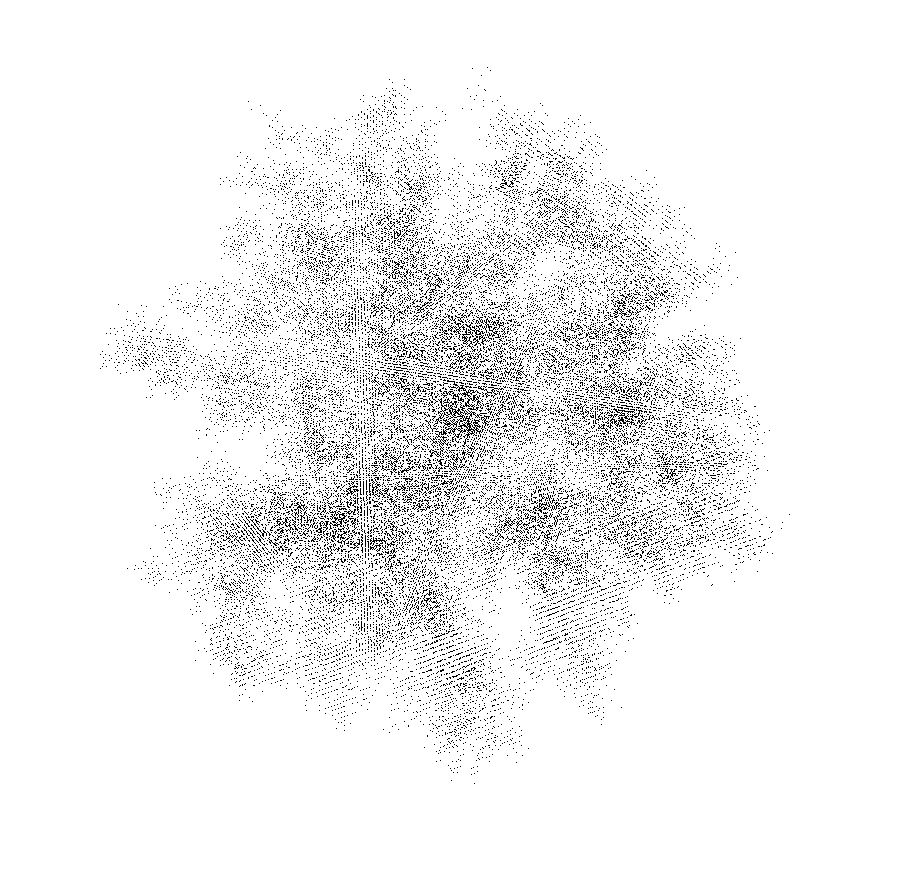
\includegraphics[width=\linewidth]{images/DLA45007-2-BW.png}
    \caption{Aggregate structure resulting from a DLA simulation using 50,000 particles. Aggregate structure shown contains 45,007 particles.}
    \label{fig:DLA45007}
    \end{figure}

%------------------------------------------------
\section{Diffusion Limited Aggregation}
Diffusion Limited Aggregation has many parallels to natural systems. Crystalline growth is a commonly used example, where particles in suspension aggregate on a structure which grows as more particles in suspension collide with the structure. Shown in Figure \ref{fig:Aggregate} from YouTube user Anne Helmenstine \cite{Helmenstine:2011} is a salt crystal she grew. This is an example of an aggregate structure, as the crystals form on the previously existing crystals in the structure.

\begin{figure}[!h]\centering % Using \begin{figure*} makes the figure take up the entire width of the page
    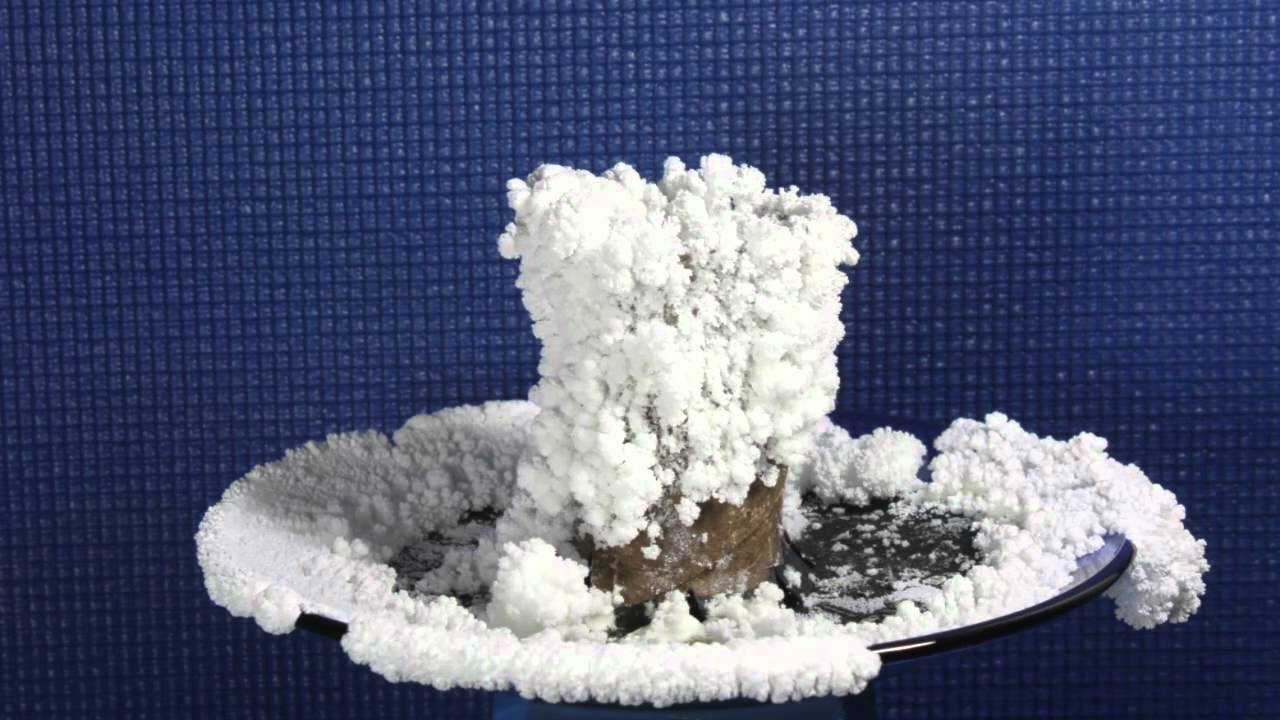
\includegraphics[width=\linewidth]{images/saltCrystal.jpg}
    \caption{In this image, taken from Anne Helmenstine's YouTube channel \cite{Helmenstine:2011}, an example of aggregate crystal growth is shown.}
    \label{fig:AnneHelmenstineSalt}
    \end{figure}

~\\

For this DLA simulation, we make several simplifications in order to ease the simulation process. For example, we do not consider aggregations between active particles. This means that there can be no "detached aggregators" which float around the simulation space aggregating particles as they go. Another such simplification that we make is that active particles not only do not aggregate with eachother, but they do not collide as well. This means that if in a given timestep two active particles move to the same location, they will occupy that location until the next timestep where they will most likely move apart from one another. In normal crystal growth, many small aggregate structures form as particles collide with eachother in solution, and then these combine to form larger aggregate structures.
\section{Implementation}
\subsection{Classes}
\subsubsection{Particle}
The \texttt{Particle} class is the most basic object of the simulation. The particle class defines only the location of the particle, the particle’s morton code, and functions to retreive/set these values. During the simulation, a particle will move randomly in one of eight possible directions by adding a random integer value [-1, 1] to each component of the particle’s position. Particles also contain a function which encodes the position into a 30-bit morton code, which is used to accelerate aggregation detection.\\

\subsubsection{Universe}
The \texttt{Universe} class is the overarching structure which contains all simulation operations. \texttt{Universe} contains an \texttt{std\allowbreak::vector} of all aggregated particles, and an \texttt{std\allowbreak::list} of all active particles. During each step of the simulation, the active particle list is iterated through, and each particle is moved, checking for collisions with the aggregate particles. For simplicity, collsions between active particles cannot occur, and the two particles will simply pass through eachother. \\~\\
Boundary conditions for the universe are enforced by not allowing a particle to travel beyond the simulation bounds. Should a particle be assigned a random motion that would take it outside of the simulation bounds, the component that would exceede the simulation bounds is capped at the bound. \\~\\
The \texttt{Universe} class also contains the visualizer launcher, which is called before the simulation begins running, and launches the visualizer in a seperate pthread task.\\

\subsection{Fast Aggregate Lookup}
To speed up collision detection with the aggregate particles, each aggregate particle is assigned a Morton code based on the position of the particle. A helpful diagram for this is shown in Figure \ref{fig:KarrasMortonGeneration} which is taken from \cite{Karras:2012}. The \texttt{std\allowbreak::vector} container which holds all aggregator particles is then sorted using the aggregator particle's morton code. \\~\\
Currently, the implementation sorts the vector of aggregate particles every timestep. A more efficient implementation of this would be to use binary insertion to place new aggregator particles into the vector. This could be efficiently achieved by using a linked list, like the Active particles are stored. Linked lists would allow for insertion without a memory movement penalty like a vector would incur. Future versions of DIGLS may implement this.\\

\begin{figure}[!h]\centering % Using \begin{figure*} makes the figure take up the entire width of the page
    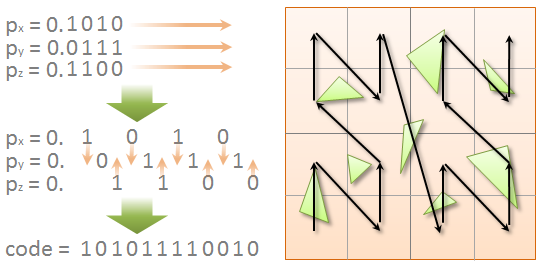
\includegraphics[width=\linewidth]{images/fig04-z-curvekarras.png}
    \caption{In this image, taken from \ref{karras2012}, the process of creating a 3 dimensional morton code using bit-interleaving is shown.}
    \label{fig:KarrasMortonGeneration}
    \end{figure}

~\\
During the collision check step, rather than search the entire aggregator particle vector looking for a particle that matches the position of the desired movement, Morton encoding allows the vector to sorted in a deterministic way, and searched using \texttt{std\allowbreak::binary\_serch}. This reduces the lookup time from $O(n)$ to $O(\log n)$ for each collision.\\

\subsection{Visualizer}
Visualization is done using OpenGL. To increase performance, the visualizer is run in a separate thread using Pthreads. When the \texttt{Universe\allowbreak::renderUniverse()} method is called, the visualizer is started, and passed a pointer to the Universe class that called the visualizer. The visualizer features some interactive features which are listed at the bottom of the simulation window. An example of the visualizer window is shown in Figure \ref{fig:DLAAPP}.
\begin{figure}[!h]\centering % Using \begin{figure*} makes the figure take up the entire width of the page
    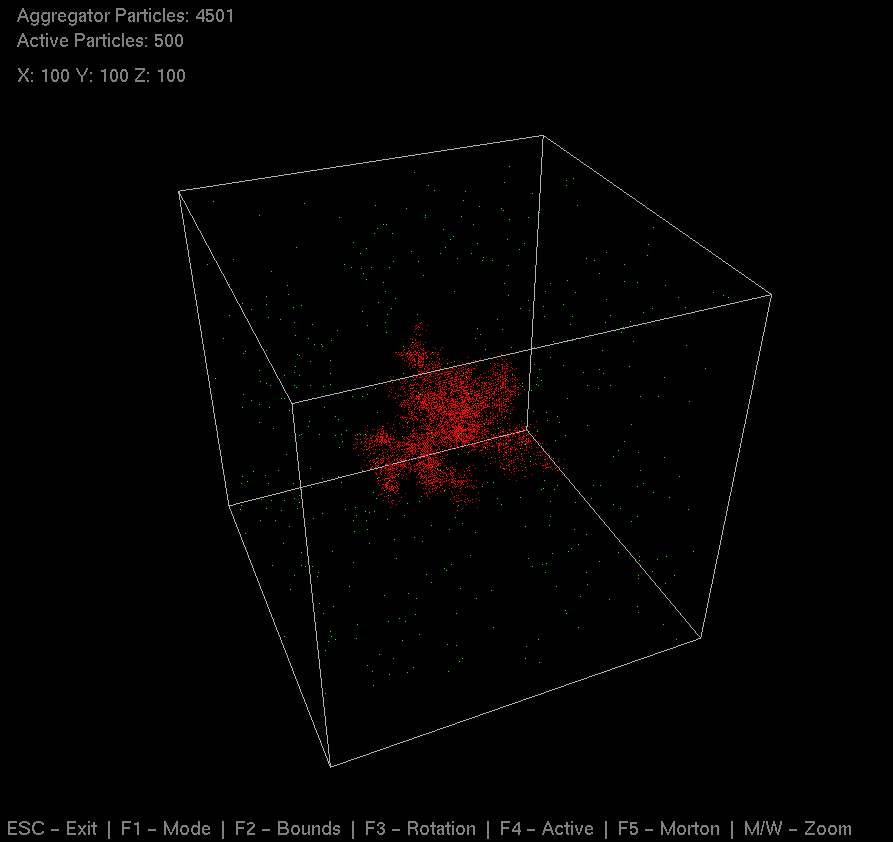
\includegraphics[width=\linewidth]{images/DLAVisualizer.png}
    \caption{DLA Visualizer application shown using fast graphics, bounding box, and active particles visible (green).}
    \label{fig:DLAAPP}
    \end{figure}

~\\
One issue that was encountered was flickering and graphic artifacting during visualization. This was discovered to be caused by sort, insertion, and deletion operations running in the simulation code while the visualizer was copying the simulation state.\\~\\
This was solved by implementing a mutex lock to prevent both threads from accessing the data at the same time. Since the visualizer and simulator will only lock resources for a short period of time, this results in no noticible effect other than a smoother simulation.\\

\subsubsection{Graphics Modes}
DIGILS features two different graphics modes: Fast and Fancy. Fast graphics renders all particles as points. Aggregator particles are shown in red, and Active particles are shown in green. Fast graphics will render each particle as a sphere, complete with local lighting effects, however visualizer performance will take a significant hit with large numbers of particles. Figure \ref{fig:Fancy} shows the simulator running in Fancy mode.

\begin{figure}[!h]\centering % Using \begin{figure*} makes the figure take up the entire width of the page
    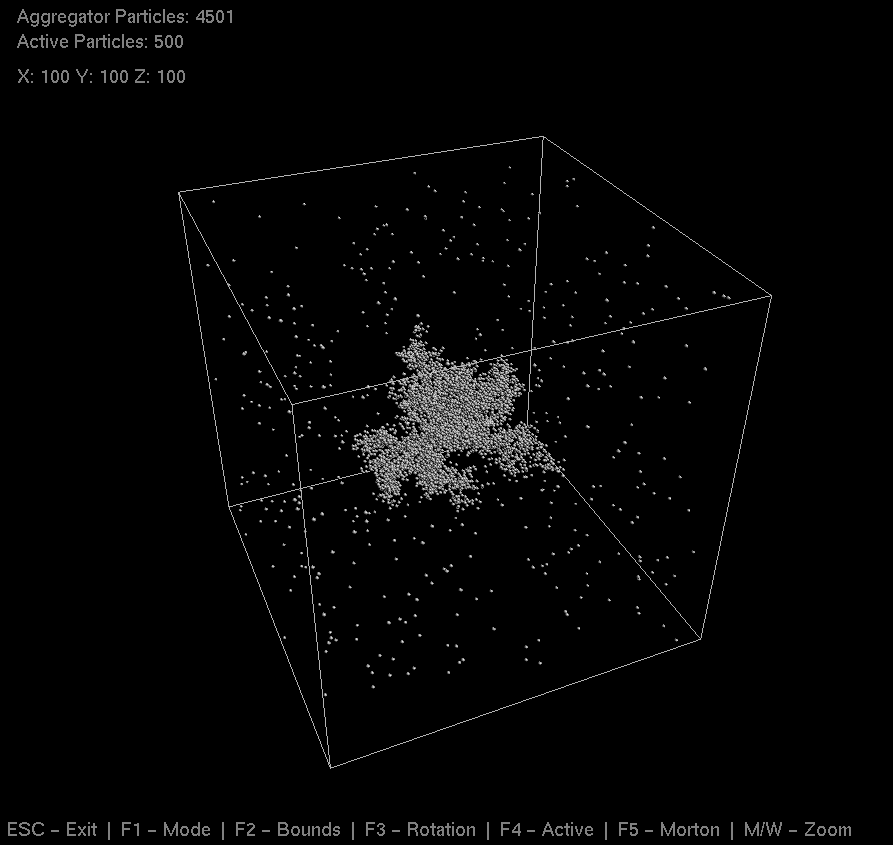
\includegraphics[width=\linewidth]{images/Fancy.png}
    \caption{DLA Visualizer application shown using Fancy graphics, and bounding box.}
    \label{fig:Fancy}
    \end{figure}

~\\
\subsubsection{Bounding Box}
By default, a bounding box is drawn around the simulation space, in order to distinguish the simulation volume from the background. Should the user desire, this bounding box may be toggled.\\

\subsubsection{Rotation}
By default, DIGILS will rotate the camera around the simulation space as the simulation progresses. Should the user desire, this rotation can be toggled on and off.\\

\subsubsection{Active Particle Display}
Active particles are not displayed by default, as this can greatly reduce visualizer performance at the beginning of a simulation should the number of particles be large. The user however may toggle the display of active particles in both Fast and Fancy graphics modes.\\

\subsubsection{Morton Line Display}
With the most recent release of DIGILS, the user may toggle on or off the morton line which the simulation uses to calculate collisions. More details about this can be found in the paper titled "Visualization of Diffusion Limited Aggregation Simulations using OpenGL". An example of the \texttt{100Corners.dat} simulation file is shown after completing a simulation, with the Morton line enabled in Figure \ref{fig:CornersMorton}.
\begin{figure}[!ht]\centering % Using \begin{figure*} makes the figure take up the entire width of the page
    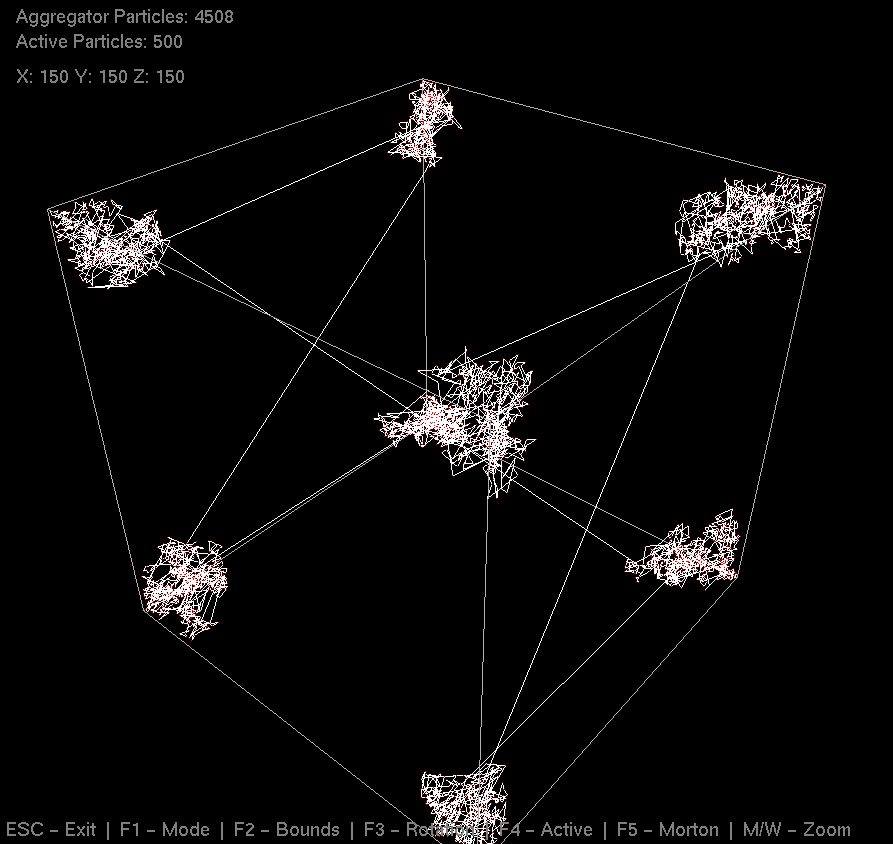
\includegraphics[width=\linewidth]{images/CornersMorton.png}
    \caption{DLA Visualizer application shown using fast graphics, bounding box, and morton line overlay.}
    \label{fig:CornersMorton}
    \end{figure}
~\\

\subsubsection{Zoom}
Using the mouse wheel, the user may adjust the position of the camera closer or farther to the simulation center (which is calculated automatically at the beginning of visualization). Zoom works by calculating an offset to add to the camera's x, y, and z positions. Each click of the mouse wheel calls a function registered with freeGLUT which increments this offset by plus or minus 10. Should the value plus the camera's default position be equal to zero, the zoom value is no longer allowed to be increased, in order to prevent zooming "through" the simulation space. Figure \ref{fig:FancyNoBound} shows the simulator zoomed in, with no bounding box displayed.\\

\begin{figure}[!ht]\centering % Using \begin{figure*} makes the figure take up the entire width of the page
    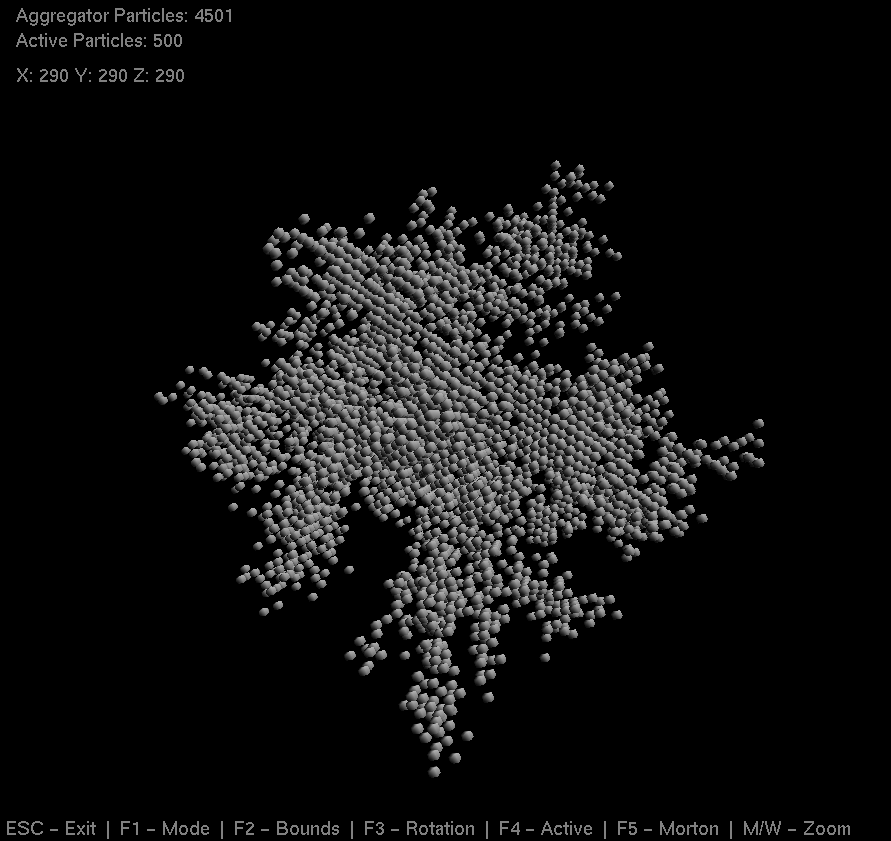
\includegraphics[width=\linewidth]{images/FancyNoBound.png}
    \caption{DLA Visualizer application shown using fancy graphics, no bounding box, no active particles, and zooming.}
    \label{fig:FancyNoBound}
    \end{figure}

freeGLUT is an open source alternative to the GL Utility Toolkit (GLUT), which is a library for C/C++, FORTRAN, and Ada. Writing a visualizer with freeGLUT consists of writing several functions and registering them with freeGLUT so that they can be executed during certain events. These include:
\begin{itemize}
    \item keyboard input
    \item mouse input
    \item window resize
    \item program idle
\end{itemize}
~\\
\subsubsection{Initialization}
    During the initialization of the visualizer, several things must be taken care of before the program can continue. First, the display mode must be set. During this tell freeGLUT that we would like to use the depth buffer, double precision values for color/position/etc. and that we are using RGBA for our color profile.\\

\subsubsection{Render Scene}
    The workhorse function in the visualizer is the \texttt{renderScene()} function which reads the universe data, and renders it for the user. \\~\\
    First, the function clears the depth buffer and the color buffer, so that we are starting with empty buffers. Next, we translate the camera, and tell it to look at the origin. We then rotate the camera around the origin by the current value specified by the rotation variable, which gets incremented each time the function is called. Next, the bounding box is drawn on the screen. Once this is complete it is time to render the particles. \\~\\
    To accomplish this, we first check which rendering mode we are using. If we are using fancy graphics, we enable lighting, otherwise we keep it disabled. We then push our matrix back onto the stack, and then translate to each location where there should be a particle, and place one there, using either a sphere or a point depending on the fancy/fast setting. If necessary, we then disable lighting, as the particles are the only object subject to lighting.\\~\\
    We then check to see if the user has requested for the morton curve to be drawn. If they have, we iterate through the list of aggregators, and create a \texttt{GL\_LINE\_STRIP} object using all of the aggregator locations as vertices. Since the aggregators are already sorted by morton code, this will result in the proper ordering of the morton curve.\\~\\
    Finally, we render the real time information on the screen by pushing the projection and model view matrices onto the stack, and then loading the identity into both. We are now free to draw text on the screen using an ortho2d projection matrix. To account for height and width changes of the window, we request values for these, and then locate our text proportionally based on the window size. Once complete, we pop the projection and modelview matrices to return to our normal view of the rest of the simulation.\\~\\
    Once all drawing tasks have completed, we increment the rotation counter, and the call \texttt{glutSwapBuffer} to swap the draw and display buffers so that the user can see the new frame.\\~\\
    The overall framework for this function can be seen in Algorithm \ref{fig:RenderFunction}.

    \begin{algorithm}
        \caption{Render Scene}\label{fig:RenderFunction}
        Clear Color Buffer\\
        Clear Depth Buffer\\
        Read Universe State\\
        Translate and Rotate Camera\\
        Draw Bounding Box\\
        \If{(fancyRender == True)}
        {
            Enable Lighting
        }
        \For{(p in particles)}
        {
            \If{(showActive == False \&\& p == Active)}
            {
                Continue
            }
            \Else
            {
                Draw Particle
            }
        }
        \If{(fancyRender == True)}
        {
            Disable Lighting
        }
        \If{(showMorton == True)}{
            START GL\_LINE\_STRIP\\
            \For{(p in particles)}
            {
                \If{p == Aggregate}
                {
                    Add Vertex p.position
                }
            }
            END GL\_LINE\_STRIP\\
        }
        Display Controls
        Display Stats
        \If{(rotation == True)}
        {
            rotationAngle += rotationIncrement 
        }
        Swap Buffers
    \end{algorithm}
    
\subsubsection{Keyboard Input}
    To enable interactivity, several options must be availabile on the keyboard. Keyboard input is enabled in freeGLUT with registration of two functions. The first function handles input of regular keys. In our case, the only regular key used is the "ESC" key, which is used to exit the visualizer. The second function is used to handle the function keys F1-F12. These are the keys that we use to control most of the interactivity of the simulation. When a function key is pressed, a global toggle corresponding to the option is toggled. For example, if a user presses "F4" a global boolean \texttt{showActive} is toggled, and is used by the \texttt{renderScene()} function to determine whether or not to draw the active particles.\\
    
\subsubsection{Mouse Input}
    To enable the user to zoom in and out of the simulation space, a mouse input function is registered with freeGLUT. When mouse input is detected, this function is called. In most cases, the mouse scroll wheel is detected as buttons 3 and 4. Each click of the mouse wheel counts as a button press and release event, so to avoid scrolling twice per tick, we ignore any \texttt{GLUT\_UP} events, and only increment the zoom offset on \texttt{GLUT\_DOWN} events, which will occur once per scroll wheel tick.\\
     
\subsubsection{Window Resize}
    When a user resizes the window, we must recompute the projection matrix, as the viewport has changed size. To do this, we register a function with freeGLUT that is called when freeGLUT detects that the window has changed size. When the function is called, we switch to the projection matrix, load the identity to clear it, and then recompute the projection matrix using the new window height and width as the viewport dimensions.\\
    
\subsubsection{Program Idle}
    When none of these functions are being used, freeGLUT will call the idle function. During idle, we would like the visualizer to continue rendering like normal, so we simply register the \texttt{renderScene()} function as the idle function.\\

%------------------------------------------------
\section{Performance Analysis}
\subsection{Simulation}
\subsubsection{Binary Collision Performance}
Shown in Figure \ref{fig:BinaryCollision} is a plot of collision lookup time vs number of particles in the simulation.
\begin{figure}[!ht]\centering % Using \begin{figure*} makes the figure take up the entire width of the page
    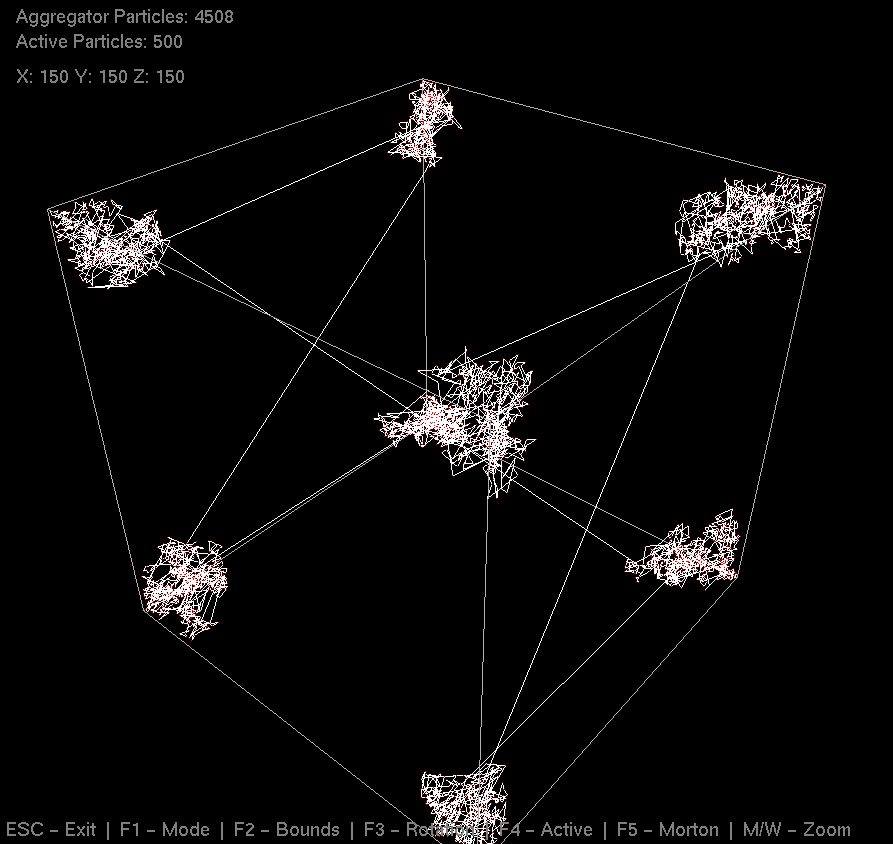
\includegraphics[width=\linewidth]{images/CornersMorton.png}
    \caption{DLA Visualizer application shown using fast graphics, bounding box, and morton line overlay.}
    \label{fig:CornersMorton}
\end{figure}

\subsection{Visualizer}
\subsubsection{Render Mode}
Shown in Figure \ref{fig:renderTime} is a comparison of render times for Fast and Fancy graphics modes vs number of particles for one frame of the visualization. 
\subsubsection{Morton Line}
Shown in Figure \ref{fig:mortonRenderTime} is a comparison of render times for Fast and Fast w/ Morton Line vs number of particles for one frame of the visualization.


%------------------------------------------------
\phantomsection
\section*{Acknowledgments} % The \section*{} command stops section numbering
Morton Encoding code taken from \cite{Karras:2012}\\
Salt structure example used from Anne Helmenstine's 2011 video \cite{Helmenstine:2011}
%----------------------------------------------------------------------------------------
%	REFERENCE LIST
%----------------------------------------------------------------------------------------
\phantomsection
\bibliographystyle{unsrt}
\bibliography{references}

%----------------------------------------------------------------------------------------

\end{document}